\documentclass[../Main.tex]{subfiles} 
\begin{document}

\section{Geo location attempt }
\subsection{Introduction}
As stated in the previous chapter, the foundation of all calculations in the regional word attempt is a list of a few hundred words that appear more likely in a specific region. 
Although this list and their probability distribution is based on scientific research it markes the weak spot of this attempt for number of reasons. For example people in a specific region use a typically word in their everyday language while speaking to their friends or family, but there is no proof that this people also use this words in their written language, even if it is only their private Twitter account. In addition, the list is way to short to cover only fraction of the words, people use on Twitter, so the end results mostly rely on the data that is generated in main loop of the algorithm.

We seem to have no other choice but to trust this generated values, so we had the idea of skipping the manually created word list and use an automatically created based on a corpus of Tweets with a geo location instead. \\
Before entering the main loop, we had to write another algorithm that learns the distribution on all seven regions for all the words in the corpus. This way we are generating a list of words that covers nearly all the words.
\begin{figure}
  \begin{center}
   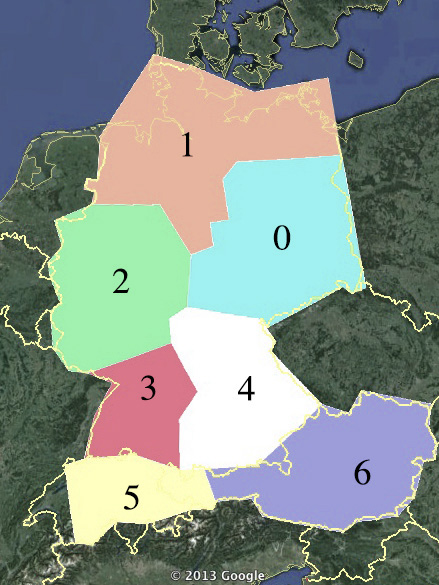
\includegraphics[width=0.5\columnwidth]{../img/polygone_satt.jpg}
    \caption{\label{geo_polymap} Map of the regions and their index represented as polygons}
  \end{center}
\end{figure}
In order to classify a tweet, that has a geo location, we had struggled to find a good way to represent the seven regions in a way, that we could easily check from which of them a Tweet was sent. After a few unsuccessful approaches, we decided to define polygons for the regions that are not overlapping each other, but also leave no gaps between them. For the value of the points we simply used their longitude and latitude coordinates, that can be represented as floats.  
We did not implement a point-in-polygon algorithm ourself, but used the version found here [SOURCE] instead. 
To find out from which region a tweet was sent, we iterate over all regions and return the first one, where the point-in-polygon function returns true.
In this first step, the Tweet-vector consists only of zeros and a one for the feature standing for the region it was sent from. 

Let's assume that the coordinates of some Tweet reveal, that its region is "Westdeutschland", represented by the index $3$.
Therefore the Tweet-vector is $(0,0,1,0,0,0,0)$. 
The next step consists of iterating over all token in the tweet and add the Tweet-vector to their word-vectors. To put it simply, we increase the counter for the specific feature of all occurring tokens by one. 
In the final step, we iterate over all word-vectors and use our \texttt{normalize()}-function to attain the probability distribution, how likely it is that the token is used in a specific region. Because of this normalization, the format of the outcome is comparable to the input list in the regional-word attempt and we can use the main part of the algorithm without having to adjust it.

\begin{figure}
\centering $\textrm{Example Tweet: } d = \textrm{'Hello Twitter!'} \textrm{ from the region 'Westdeutschland'.}$
 \begin{align*}
    \vec{t}_{hello} &= (1,3,2,5,2,1,0) \\
     \vec{t}_{twitter} &= (0,0,0,0,0,0,0) \\
      \vec{d} &= (0,0,1,0,0,0,0) \\
     \vec{t}_{hello}' &= \vec{t}_{hello} + \vec{d} =  (1,3,3,5,2,1,0) \\
    \vec{t}_{twitter} ' &= \vec{t}_{twitter} + \vec{d} = (0,0,1,0,0,0,0) \\
     \texttt{normalize(}\vec{t}'_{hello}\texttt{)} &= (0.04, 0.13, 0.13, 0.22, 0009, 0.04, 0) \\
     \texttt{normalize(}\vec{t}'_{twitter}\texttt{)} &= (0,0,1,0,0,0,0)
  \end{align*}
  \caption{Example for the creation of the initial word-vectors}
  \label{geo_example1}
\end{figure}

\subsection{Source of data}
The datasets used for the generation of the first word-vectors have been extracted from the Scheffler-corpus using the same classification function as in the main program. Although the corpus mostly consist of German Tweets (filtered with \emph{LangID}), about 20\% of the Tweets with geo-location have not been sent from one of the defined regions and therefore have been ignored. \\
We created balanced sets, where the amount of  Tweets are the same for all regions. Because the fewest number of Tweets (8787) came from region 6, 'Austria', we ended up with only 61509 Tweets for all regions. 

In order to create a gold-standard, we substracted 150 Tweets from each region, leaving us 60459 for the training. \\
Our assumption was, that datasets of different sizes lead to different results and we wondered, how it would effect the accuracy, if we would use the same data for the creation of the word-vectors and for the main-algorithm. Therefore we created three balanced sets, one unbalanced set of all geo annotated Tweets and as a reference one huge set of normal Tweets. Of course none of these sets contain any Tweets from the gold-standard-set.
 \begin{enumerate}
\item \emph{balanced-21k} with 3000 Tweets from each region.
\item \emph{balanced-39k} consisting of the remaining 39456 Tweets
\item \emph{balanced-61k} combining the both previous sets. 
\item \emph{geo-175k} with all Tweets from the corpus that were sent from one of the defined regions. Not balanced.
\item \emph{all-1500k} contains 1.5 million mostly not geo annotated Tweets.
\end{enumerate}
\subsection{Experiments}
\subsubsection{Dataset combinations}
\begin{table}[b]
    \begin{tabular}{|l|lllll|}
    \hline
    Geo dataset     & balanced-21k & balanced-39k & balanced-61k & geo-175k & all-1500k \\ \hline
    balanced-21k    & 0.319        & 0.308        & 0.304        & 0.307           & 0.308       \\
    balanced-39k    & 0.306        & 0.353       & \textbf{0.345}        & \textbf{0.368 }          & 0.306       \\
    balanced-61k    & \textbf{0.336}        & \textbf{0.361}        & 0.344        &0.360           & 0.332       \\
    unbalanced-175k & 0.303        & 0.343        & 0.322        & 0.352           & \textbf{0.340}       \\ \hline
    \end{tabular} \\

  Calculation method: \textit{Normalized}; Stopwords: \textit{Top 200}; Loops: \textit{1}; Estimated amount of non-regional Tweets: \textit{60\%}, leading to a similarity threshold between \textit{0.999} and \textit{0.991}, depending on the dataset.
  \caption{Comparrision of the combination of all datasets}
  \label{geo_datasets}
\end{table}

In order to give a solid foundation which data we should use in further experiments, we started to compare the combination of the five datasets we created. We wondered, how it would affect the accuracy, if we would for example train the geo-algorithm with a small set of geo-annotated data but use a very big set of Tweets for the learning of the word-vectors in the loop of the main-algorithm. Another question was, what results we would get, if the data in the main-algorithm contains Tweets, that have been used in the geo-algorithm before. 

Our expectation was in general, that the accuracy would rise, the more data we use and that the reuse of Tweets in the main-algorithm would lower it, because this data already had an effect and using it again would not change anything.

Unsurprisingly, using the smallest set, \emph{balanced-21k}, for the training of the geo-algorithm nearly always produced the lowest accuracy. \\
But our hypothesis about the reuse of data was falsified:  The combination of the \emph{balanced-39k} set for the learning in the geo-algorithm and \emph{balanced-61k} for the main-algorithm generated the third best result with an accuracy of 0.345.

Also we discovered, that the use of balanced data  in the geo-algorithm, where all regions are represented by the same amount of documents, is crucial for good results. Having a look at the row for the \emph{unbalanced-175k}, it produces a very bad accuracy. Even in combination with the set containing 1.5 million Tweets (\emph{all-1500k}), it marks the second last rank.

This experiment showed us, that we should use the \emph{balanced-39k}-set for the training of the geo-algorithm and the \emph{geo-175k}-set for the main-algorithm, because it generated the best accuracy of 0.365. We were surprised, that the combination \emph{balanced-39k} / \emph{all-1500k} had a worse result, but interpreted it as a result of the unfiltered data of the \emph{all-1500k}-set.

\subsubsection{Comparission of different stopword-lists}
\begin{figure}
\begin{center}
\begin{tikzpicture}
        \begin{axis}[
                              width=0.9\columnwidth,
                              height=0.3\textheight,
                              symbolic x coords={0, 100, 200, 500, 750, 1000},
                              xtick=data,
                              ytick={0.26, 0.28, 0.3,0.32, 0.34,0.36, 0.38},
                              ylabel=accuracy,
                              bar width=40,
                              xlabel=number of stopwords
          ]
            \addplot[ybar,  postaction={ pattern=north east lines  }] coordinates {
               (0, 0.2762)
               (100, 0.352)
               (200, 0.368)
	      (500, 0.333)
               (750, 	0.318)
               (1000, 0.299)
            };
        \end{axis}
    \end{tikzpicture}
\end{center}
  \label{geo_graph1}
Calculation method: \textit{Normalized}; Geo-dataset: \textit{balanced-39k}, Main-dataset: \textit{geo-175k}; Loops: \textit{1}; Estimated amount of regional Tweets: \textit{60\%}
  \caption{Accuracy of different stopword-lists.}

\end{figure}

Zipf's law tells us that a very small amount of token are found extremely often in corpora, while most token appear only a few times. Because it is much more likely for a more seldom word to have a regional meaning, we decided to filter out the most frequent token. 

We came up with the idea, that it is not reasonable to use a existing stopword-list for the German language because people on Twitter could use specific words more often than for example in a standard German text. In addition, spam bots or automatically sent messages, that always contain the same words, are extremely often and  have to be filtered. So we used the Scheffler corpus to create our own stopword-list by using our modified version of Christopher Potts' tokenizer and counting the frequency of all token.

We were unsure, how many token should be appear on a stopword-list, so we created five of them, containing the most \emph{100}, \emph{200}, \emph{500}, \emph{750} and \emph{1000} frequent words.\\
Actually, we expected the have a better accuracy, the more stopwords we use, but he have been proved otherwise. 
Figure \ref{geo_graph1} show clearly, that more than 200 stopwords lead to a worse results, while only 100 stopwords also have a lower accuracy (0.352) than the list containing 200 entries (0.368). The fact, that the results of the run with no stopword filtering at all had the lowest accuracy (0.276), reveals the importance of the use of a stopword-list.\\
Because the list containing 200 stopwords lead to the best results, we will use this one in further experiments.

\subsubsection{Guessing the amount of regional Tweets}
\begin{figure}
\begin{tikzpicture}
       \pgfplotstableread{../data/geo_cos.csv}\data
       \begin{axis}[
           legend pos=south east,
           ylabel near ticks,
           axis y line*=left,
           xmin = 5,
           xmax = 100,
           ylabel= accuracy,
           xlabel= guessed percentage of non-regional Tweets,
           xtick = {5,10,20,30,40,50,60,70,80,90,100},
           width=0.9\columnwidth,
           height=0.5\textheight]
           \addplot[blue, mark=x] 
           table[x=Guess,y=Accuracy]{\data} ;
           \addlegendentry[font=\tiny]{accuracy}
       \end{axis}
       \begin{axis}[
           hide x axis,
           xmin = 5,
           xmax = 100,
           axis y line*=right,
           legend pos=south west,
           ylabel near ticks,
           ylabel= cosine similarity threshold,
           width=0.9\columnwidth,
           height=0.5\textheight]
           \addplot[red, mark=x] 
           table[x=Guess,y=Threshold]{\data};
           \addlegendentry[font=\tiny]{threshold}
       \end{axis}
\end{tikzpicture}
Calculation method: \textit{Normalized}; Geo-dataset: \textit{balanced-39k}, Main-dataset: \textit{geo-175k}; Stopwords: \textit{Top 200}; Loops: \textit{1}; 

  \caption{Relation between the amount of regional Tweets and the accuracy.}
  \label{geo_graph2}
\end{figure}
In section 2, 'Algorithms', we talked about the advantages and disadvantages of filtering too ordinary Tweets using the cosine similarity metric. Summarized, we gain much better results, considering the accuracy, but have to accept, that we cannot classify a huge percentage of Tweets, because they do not differ enough from the average Tweet-vector.

We wanted to know, what high the accuracy could be, so ran the program a few times, changing the parameter guessing the amount of regional Tweets. We started at 100\% and went down to an extreme of 5\%.

The results approved our hypothesis, as the accuracy rises, the lower we guess. Of course, the similarity threshold lowers to values of 0.92 at a guess of 5\%. \\
The highes accuracy we could archive had a value of 0.506, guessing that only 20\% of all Tweets are regional salient. We were extremely happy about this result, as we started our first experiments with an accouracy as low as about 0.2, but we had to keep in mind that 80\% of all Tweet will be ignored. If we lower our guessing to 10\% or 5\%, the accuracy gets lower again, probably because there are not enough Tweets left in the gold-standard to give an trustworthy result. 

There is no ideal value for this parameter and eventually, people who would use this algorithm have to figure it out themself, according to what they want to archive: A higher coverage of data or a more reliable result. \\
In further experiments, we decided to use a guessing of 20\%, because our aim is to get the highest accuracy as possible.

\subsubsection{The right amount of loops}
\begin{figure}
\begin{tikzpicture}
       \pgfplotstableread{../data/geo_loops.csv}\data
       \begin{axis}[
           legend pos=south east,
           ylabel near ticks,
           xmin = 0,
           xmax = 20,
           ylabel= accuracy,
           xlabel= loops,
           xtick = {0,1,2,3,4,5,10,15,20},
           width=0.9\columnwidth,
           height=0.4251174\textheight]
           \addplot[blue, mark=x] 
           table[x=Loops,y=Accuracy]{\data} ;
       \end{axis}
\end{tikzpicture}

Calculation method: \textit{Normalized}; Geo-dataset: \textit{balanced-39k}, Main-dataset: \textit{geo-175k}; Stopwords: \textit{Top 200}; Estimated amount of regional Tweets: \textit{20\%}
  \caption{Amount of loops in the algorithm and their effect on the accuracy.}
  \label{geo_graph3}
\end{figure}
The idea between in the loops in the main-algorithm was to estimate the probability distinction from which region a tweet could have been set to as many words as possible. This was especially for the regional-list attempt a crucial approach to prevent the sparse data problem.

In this attempt on the other hand, this problem is not so urgent, because we create a very large list of word-vectors based on geo-annotated data. Therefore we asked ourself, which amount of loops would lead to the best results. The more the better or the opposite? 

To find an answer to this question, we chose the parameters we had proven to be the best choice in the experiments before, but varied to value for the loop-parameter from 0 to 20 and measured the accuracy. 
We were a bit puzzled to find out, that the main loop, even if it was only ran once, lowers the accuracy by 0.023. Our new record for the accuracy becomes 0.53, if we use a value of 0. 

If we have a look at the graph in figure \ref{geo_graph3}, we can clearly see that the accuracy drastically decreases, the more loops we enter. So our assumption, that the loops in the main-algorithm would lead to better results has been falsified. We now came up with the explanation, that the more often we use a loop, the more do all word-vectors approach an average word-vector and in this way lose all signs of a specific region.

In addition to finding out the best value for the loops runs, we now know, that the parameter for the second dataset, that was relevant for the training in the main-algorithm, has only the purpose of a foundation for creating the cosine similarity. This also raises the question, whether our results in the first experiment 1.3.1, are still valid. So we ran the experiment with the loops=0 setting again.

The results were slightly different than before, ranking the \emph{balanced-61k} as the best dataset for the training of the geo-algorithm. To be sure that the outcomes of the other experiments are still valid, we made some spot checks that showed, that the values differ a little bit, but the end results were still the same. In further experiments, we now use the settings "loops=\emph{0}" and "geo-dataset=\emph{balanced-61k}"
\begin{table}
\begin{center}
    \begin{tabular}{|l|llll|}
    \hline
    Dataset     & balanced-21k & balanced-39k & balanced-61k & geo-175k \\ \hline
    Accuracy    & 0.339       & 0.342        & \textbf{0.364 }       & 0.332                \\ \hline
    \end{tabular} \\
\end{center}
  Calculation method: \textit{Normalized}; Stopwords: \textit{Top 200}; Loops: \textit{0}; Estimated amount of non-regional Tweets: \textit{60\%}.
  \caption{Comparrision of the accuracy for all geo-datasets with a loop parameter of '0'}
  \label{geo_datasets}
\end{table}

\subsubsection{Comparission of different calculation methods}
\begin{figure}
\begin{center}
\begin{tikzpicture}
        \begin{axis}[
                              width=0.9\columnwidth,
                              height=0.3\textheight,
                              symbolic x coords={Normalized, Sqrt, Log, Linear},
                              xtick=data,
                              ylabel=accuracy,
                              bar width=40,
			 ymin=0.25,
			 ymax=0.6,
			ytick={0.25,0.35,0.45,0.55},
			 nodes near coords,
    			  nodes near coords align={vertical}
          ]
            \addplot[ybar,  postaction={ pattern=north west lines  }] coordinates {
               (Normalized, 0.539)
               (Sqrt, 0.330)
               (Log, 0.265)
	      (Linear, 0.365)
            };
        \end{axis}
    \end{tikzpicture}
\end{center}
  \label{geo_graph1}
Calculation method: \textit{Normalized}; Geo-dataset: \textit{balanced-39k}, Main-dataset: \textit{geo-175k}; Loops: \textit{1}; Estimated amount of regional Tweets: \textit{60\%}
  \caption{Accuracy of different stopword-lists.}

\end{figure}


As mentioned in the 'Algorithms'-section before, we developed four different versions of the algorithms, that differ mostly in the way of normalization. We named our first attempt, that we also used in the previous experiments, \emph{Normalized}, the other calculation methods are \emph{Log}, \emph{Root} and \emph{Linear}. For a discussion of the details of the algorithms, please have a look at the corresponding section. 

The parameter for the calculation method is the last one we have to find an optimal value for. As recommended in the experiments before, we choosed the \emph{balanced-61k} set for the geo-algorithm, the \emph{unbalanced-175k} dataset as a foundation for the calculation of the cosine similarity, which depends on our guess of the amount of regional Tweets which we  decided to be \emph{20\%}. The amount of loops is \emph{0} and we filtered using the \emph{200} most used token as stopword-list.


%\subsection{Conclusion}

\end{document}
